% Created by tikzDevice version 0.12.6 on 2024-11-10 11:15:44
% !TEX encoding = UTF-8 Unicode
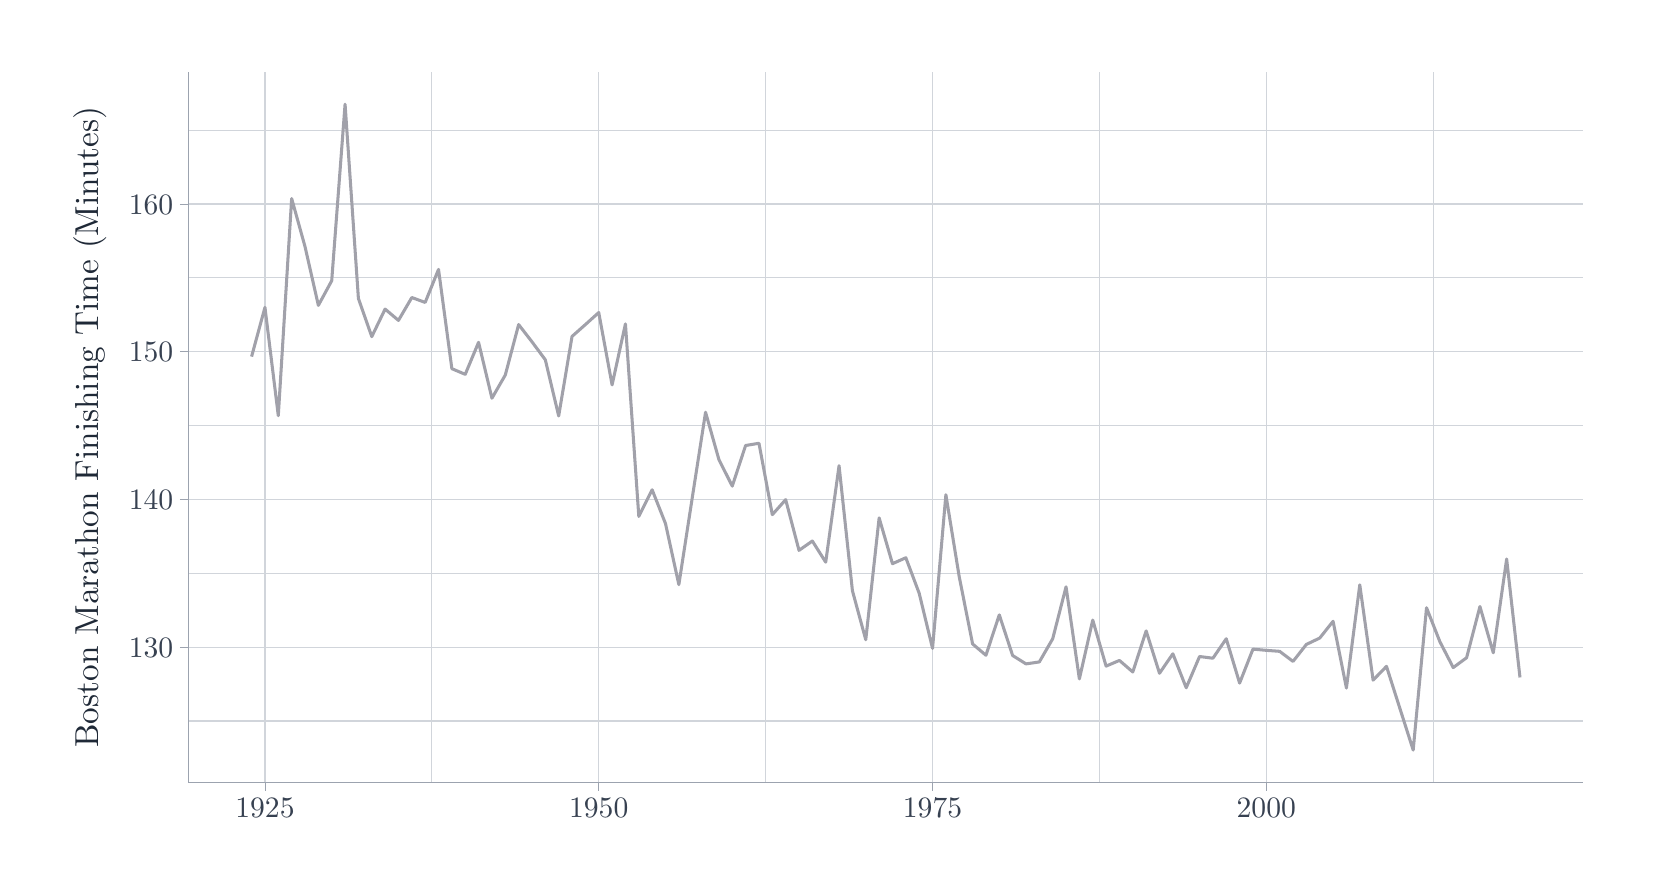
\begin{tikzpicture}[x=1pt,y=1pt]
\definecolor{fillColor}{RGB}{255,255,255}
\path[use as bounding box,fill=fillColor] (0,0) rectangle (578.16,303.53);
\begin{scope}
\path[clip] (  0.00,  0.00) rectangle (578.16,303.53);
\definecolor{drawColor}{RGB}{255,255,255}

\path[draw=drawColor,line width= 0.6pt,line join=round,line cap=round,fill=fillColor] (  0.00,  0.00) rectangle (578.16,303.53);
\end{scope}
\begin{scope}
\path[clip] ( 58.00, 30.82) rectangle (562.16,287.53);
\definecolor{drawColor}{RGB}{255,255,255}
\definecolor{fillColor}{RGB}{255,255,255}

\path[draw=drawColor,line width= 0.6pt,line join=round,line cap=round,fill=fillColor] ( 58.00, 30.82) rectangle (562.16,287.53);
\definecolor{drawColor}{RGB}{209,213,219}

\path[draw=drawColor,line width= 0.4pt,line join=round] ( 58.00, 52.99) --
	(562.16, 52.99);

\path[draw=drawColor,line width= 0.4pt,line join=round] ( 58.00,106.37) --
	(562.16,106.37);

\path[draw=drawColor,line width= 0.4pt,line join=round] ( 58.00,159.76) --
	(562.16,159.76);

\path[draw=drawColor,line width= 0.4pt,line join=round] ( 58.00,213.14) --
	(562.16,213.14);

\path[draw=drawColor,line width= 0.4pt,line join=round] ( 58.00,266.52) --
	(562.16,266.52);

\path[draw=drawColor,line width= 0.4pt,line join=round] (146.05, 30.82) --
	(146.05,287.53);

\path[draw=drawColor,line width= 0.4pt,line join=round] (266.66, 30.82) --
	(266.66,287.53);

\path[draw=drawColor,line width= 0.4pt,line join=round] (387.27, 30.82) --
	(387.27,287.53);

\path[draw=drawColor,line width= 0.4pt,line join=round] (507.88, 30.82) --
	(507.88,287.53);

\path[draw=drawColor,line width= 0.4pt,line join=round] ( 58.00, 79.68) --
	(562.16, 79.68);

\path[draw=drawColor,line width= 0.4pt,line join=round] ( 58.00,133.07) --
	(562.16,133.07);

\path[draw=drawColor,line width= 0.4pt,line join=round] ( 58.00,186.45) --
	(562.16,186.45);

\path[draw=drawColor,line width= 0.4pt,line join=round] ( 58.00,239.83) --
	(562.16,239.83);

\path[draw=drawColor,line width= 0.4pt,line join=round] ( 85.74, 30.82) --
	( 85.74,287.53);

\path[draw=drawColor,line width= 0.4pt,line join=round] (206.35, 30.82) --
	(206.35,287.53);

\path[draw=drawColor,line width= 0.4pt,line join=round] (326.97, 30.82) --
	(326.97,287.53);

\path[draw=drawColor,line width= 0.4pt,line join=round] (447.58, 30.82) --
	(447.58,287.53);
\definecolor{drawColor}{RGB}{161,161,170}

\path[draw=drawColor,line width= 1.1pt,line join=round] ( 80.91,184.67) --
	( 85.74,202.46) --
	( 90.56,163.32) --
	( 95.39,241.79) --
	(100.21,224.44) --
	(105.04,203.18) --
	(109.86,212.07) --
	(114.69,275.87) --
	(119.51,205.67) --
	(124.34,191.88) --
	(129.16,201.84) --
	(133.98,197.75) --
	(138.81,206.02) --
	(143.63,204.24) --
	(148.46,216.17) --
	(153.28,180.31) --
	(158.11,178.26) --
	(162.93,189.83) --
	(167.76,169.63) --
	(172.58,178.00) --
	(177.41,196.24) --
	(182.23,190.01) --
	(187.05,183.51) --
	(191.88,163.23) --
	(196.70,191.96) --
	(201.53,196.24) --
	(206.35,200.59) --
	(211.18,174.44) --
	(216.00,196.50) --
	(220.83,126.93) --
	(225.65,136.54) --
	(230.47,124.35) --
	(235.30,102.28) --
	(240.12,133.51) --
	(244.95,164.56) --
	(249.77,147.48) --
	(254.60,137.87) --
	(259.42,152.55) --
	(264.25,153.35) --
	(269.07,127.55) --
	(273.90,132.98) --
	(278.72,114.65) --
	(283.54,118.03) --
	(288.37,110.38) --
	(293.19,145.25) --
	(298.02,100.06) --
	(302.84, 82.35) --
	(307.67,126.39) --
	(312.49,109.84) --
	(317.32,111.98) --
	(322.14, 99.17) --
	(326.97, 79.24) --
	(331.79,134.76) --
	(336.61,105.13) --
	(341.44, 80.84) --
	(346.26, 76.75) --
	(351.09, 91.34) --
	(355.91, 76.66) --
	(360.74, 73.63) --
	(365.56, 74.34) --
	(370.39, 82.71) --
	(375.21,101.48) --
	(380.03, 68.20) --
	(384.86, 89.47) --
	(389.68, 72.83) --
	(394.51, 74.88) --
	(399.33, 70.70) --
	(404.16, 85.55) --
	(408.98, 70.25) --
	(413.81, 77.28) --
	(418.63, 65.00) --
	(423.46, 76.30) --
	(428.28, 75.68) --
	(433.10, 82.71) --
	(437.93, 66.69) --
	(442.75, 78.97) --
	(447.58, 78.53) --
	(452.40, 78.17) --
	(457.23, 74.52) --
	(462.05, 80.66) --
	(466.88, 82.97) --
	(471.70, 89.02) --
	(476.52, 64.91) --
	(481.35,102.19) --
	(486.17, 67.76) --
	(491.00, 72.74) --
	(495.82, 57.62) --
	(500.65, 42.49) --
	(505.47, 93.92) --
	(510.30, 81.64) --
	(515.12, 72.30) --
	(519.95, 75.86) --
	(524.77, 94.36) --
	(529.59, 77.64) --
	(534.42,111.53) --
	(539.24, 68.74);
\end{scope}
\begin{scope}
\path[clip] (  0.00,  0.00) rectangle (578.16,303.53);
\definecolor{drawColor}{RGB}{156,163,175}

\path[draw=drawColor,line width= 0.3pt,line join=round] ( 58.00, 30.82) --
	( 58.00,287.53);
\end{scope}
\begin{scope}
\path[clip] (  0.00,  0.00) rectangle (578.16,303.53);
\definecolor{drawColor}{RGB}{55,65,81}

\node[text=drawColor,anchor=base east,inner sep=0pt, outer sep=0pt, scale=  1.07] at ( 52.60, 76.01) {130};

\node[text=drawColor,anchor=base east,inner sep=0pt, outer sep=0pt, scale=  1.07] at ( 52.60,129.39) {140};

\node[text=drawColor,anchor=base east,inner sep=0pt, outer sep=0pt, scale=  1.07] at ( 52.60,182.77) {150};

\node[text=drawColor,anchor=base east,inner sep=0pt, outer sep=0pt, scale=  1.07] at ( 52.60,236.16) {160};
\end{scope}
\begin{scope}
\path[clip] (  0.00,  0.00) rectangle (578.16,303.53);
\definecolor{drawColor}{RGB}{156,163,175}

\path[draw=drawColor,line width= 0.3pt,line join=round] ( 55.00, 79.68) --
	( 58.00, 79.68);

\path[draw=drawColor,line width= 0.3pt,line join=round] ( 55.00,133.07) --
	( 58.00,133.07);

\path[draw=drawColor,line width= 0.3pt,line join=round] ( 55.00,186.45) --
	( 58.00,186.45);

\path[draw=drawColor,line width= 0.3pt,line join=round] ( 55.00,239.83) --
	( 58.00,239.83);
\end{scope}
\begin{scope}
\path[clip] (  0.00,  0.00) rectangle (578.16,303.53);
\definecolor{drawColor}{RGB}{156,163,175}

\path[draw=drawColor,line width= 0.3pt,line join=round] ( 58.00, 30.82) --
	(562.16, 30.82);
\end{scope}
\begin{scope}
\path[clip] (  0.00,  0.00) rectangle (578.16,303.53);
\definecolor{drawColor}{RGB}{156,163,175}

\path[draw=drawColor,line width= 0.3pt,line join=round] ( 85.74, 27.82) --
	( 85.74, 30.82);

\path[draw=drawColor,line width= 0.3pt,line join=round] (206.35, 27.82) --
	(206.35, 30.82);

\path[draw=drawColor,line width= 0.3pt,line join=round] (326.97, 27.82) --
	(326.97, 30.82);

\path[draw=drawColor,line width= 0.3pt,line join=round] (447.58, 27.82) --
	(447.58, 30.82);
\end{scope}
\begin{scope}
\path[clip] (  0.00,  0.00) rectangle (578.16,303.53);
\definecolor{drawColor}{RGB}{55,65,81}

\node[text=drawColor,anchor=base,inner sep=0pt, outer sep=0pt, scale=  1.07] at ( 85.74, 18.07) {1925};

\node[text=drawColor,anchor=base,inner sep=0pt, outer sep=0pt, scale=  1.07] at (206.35, 18.07) {1950};

\node[text=drawColor,anchor=base,inner sep=0pt, outer sep=0pt, scale=  1.07] at (326.97, 18.07) {1975};

\node[text=drawColor,anchor=base,inner sep=0pt, outer sep=0pt, scale=  1.07] at (447.58, 18.07) {2000};
\end{scope}
\begin{scope}
\path[clip] (  0.00,  0.00) rectangle (578.16,303.53);
\definecolor{drawColor}{RGB}{31,41,55}

\node[text=drawColor,rotate= 90.00,anchor=base,inner sep=0pt, outer sep=0pt, scale=  1.20] at ( 25.43,159.18) {Boston Marathon Finishing Time (Minutes)};
\end{scope}
\end{tikzpicture}
